	\section{Задачи}
		\subsection{1}
		\textbf{Корректность определения сравнения, суммы и произведения действительных чисел}
		\\
		Если одно из чисел $x,\ y$ или оба -- конечные десятичные дроби, то результат сравнения не зависит от того, какое из двух представлений (с периодом $0$ или с периодом $9$) выбрано.\\		
		Пусть $y = b_0.b_{1}b_{2}...\ , $
		
		\subsection{2}
		Определение точной верхней и точной нижней граней ограниченного числового множества. Существование точной верхней грани (как следствие из аксиомы непрерывности). Единственность точней верхней грани.
		\\
		1. A - множество ограниченное сверху. \\
		Число $d \in R $ называется точной верхней гранью (супремумом) множества $А$, если: \\
		1) d - верхняя грань \\
		2) $\forall c < d $ не является верхней гранью для $А$ \\
		Иначе говоря, $d = \sup A$, если:\\
		1) $\forall a \in A$, $ a \leqslant d $ \\
		2) $\forall c < d \ \exists a \in A$, $a > c $\\
		\\
		2. \textbf{У ограниченного сверху мн-ва существует супремум.}\\
		Рассмотрим $В$ = \{мн-во всех верхних граней мн-ва А\}
		= $\{b \in \mathbb{R} | \forall a \in A, a \leqslant b \}$, $A,B \neq \emptyset$ \\
		По аксиоме (14): $\exists d \in \mathbb{R}$ : $ a \leqslant d \leqslant b \Rightarrow d$ - $\sup A$ \\
		Возьмем $ c < d$: Допустим, что $с$ - верхняя грань, тогда $ с \in B$, \\
		но $\forall b \in B \ b \geqslant d \Rightarrow c \geqslant d $. \\
		Противоречие. \\
		\\
		3. \textbf{Супремум единственный}\\
		Пусть множество A имеет 2 точных верхних грани: $ a_1 $ и $ a_2$.\\
		Допустим, что $ a_1 < a_2$. Так как $a_1 < a_2$ и $a_2$ = supA, то $\exists a' \in A$: a' > $ a_1$, что противоречит тому факту, что $ a_1 = \sup A$.
		
		
		\subsection{3}
		\begin{gather*}
		m + n = n + m\\
		m \cdot n = n \cdot m\\
		m + (n + l) = (m + n) + l = m + n + l
		m \cdot (n \cdot l) = (m \cdot n) \cdot l = m \cdot n \cdot l
		\end{gather*}
		По аксиомам индукции:\\
		определим $x'$ как элемент, следующий за $x$\\
		для сложения 
		\begin{gather*}
			\forall a,b \in \mathbb{N}\\
			a + 1 = a'\\
			a + b' = (a + b)'
		\end{gather*}
		для умножения
		\begin{gather*}
			\forall a,b \in \mathbb{N}\\
			a \cdot 0 = 0 \cdot a = 0\\
			a \cdot 1 = a\\
			a \cdot b' = a \cdot b + a
		\end{gather*}
		
		\subsection{4}
		
		\subsection{5}
		\textbf{Композиция непрерывных отображений непрерывна}
		\\
		Если $a, b, c \subset \mathbb{R}$, функция f непрерывна в точке $a \in A$, а функция g непрерывна в точке $f(a) \in B$, то функция $g \circ f$ непрерывна в точке a.\\
		\\
		Пусть $U$ -- произвольная окрестность точки $(g \circ f)(a) = g(f(a))$. Поскольку $g$ непрерывна в точке $f(a)$, существует окрестность $W$ точки $f(a)$ такая, что если $y \in B \cap W$, то $g(y) \in U$. Но функция $f$ непрерывна в точке $a$, поэтому найдется окрестность $V$ точки a такая, что если $x \in V$, то $f(x) \in W$. Следовательно, если $x \in V$, то $(g \circ f)(x) = g(f(x)) \in U$, что и означает непрерывность.\\
		\\
		Так как мы выбрали произвольную точку $a \in A$, повторив такое рассуждение для всех точек a из $A$, мы получим, что если функции $f$ и $g$ непрерывны, то и их композиция непрерывна. 
		
		\subsection{6}
		\textbf{Единственность предела}
		\\
		Пусть $X,\ B$ -- хаусдорфовы топологические пространства, $A \subset X,\ f: A \ \Rightarrow \ B$ -- отображение, $a \in x$, $a \in A$ не изолирована в множестве $A \cup \{a\} \subset X: \forall$ окрестности $V(a) \subset X \exists b \in V \cap A \setminus \{a\}$, то есть $\exists b \in V: b \in A, b \neq a$. Тогда если существует предел $\lim_{x\to a} f(x) \in B$, то он единственный.\\ 
		\\
		Доказательство. Пусть $u_1, u_2$ -- пределы, $u_1 \neq u_2$. Из свойства Хаусдорфова пространства $\exists U_1(u_1),\ U_2(u_2): U_1 \cap U_2 = \emptyset$.\\
		Из определения предела: $\exists V_1, V_2: x_1 \in \mathring V_{1}(a) \ \Rightarrow \ f(x_1) \in U_1, x_2 \in \mathring V_{2}(a) \ \Rightarrow \ f(x_2) \in U_2$.\\ 
		\\
		$x \in \mathring V_{1}(a), x \in \mathring V_{2}(a) \ \Rightarrow \ \exists V: V \subset \mathring V_{1} \cap \mathring V_{2}$.\\ 
		\\
		Из условия $a \in A \cup \{a\}$ не изолирована $\ \Rightarrow \ \exists x \in V \cap A \neq a, x \in \mathring V_{1} \cap \mathring V_{2} \ \Rightarrow \ f(x) \in U_1, f(x) \ \in \ U_2 \ \Rightarrow \ f(x) \in U_1 \cup U_{2} = \emptyset \ \Rightarrow \ $ предел единственен. 
		
		\subsection{7}
		\textbf{Декартово произведение хаусдорфовых топологических пространств -- хаусдорфово топологическое пространство}
		\\
		Для всех $a \in X, b \in Y$ окрестностью точки $(a, b) \in X \times Y$ называется множество $U(a) \times V(b) = \{(x, y)\ |\ x \in U(a),\ y \in V(b)\}$, где $U(a) \subset X, V(b) \subset Y$ -- произвольные окрестности точек $a$ и $b$ соответственно.\\ 
		
		\subsection{8}
		
		\subsection{9}
		1) \textbf{Функция $f(x, y) = x + y$ непрерывна}
		\\
		Рассмотрим $f: \mathbb{R}^2 \ \Rightarrow \ \mathbb{R}$. Как мы знаем, функция непрерывна в точке $a$, если для любой окрестности точки $f(a)$ существует такая окрестность точки $a$, что, если $x$ лежит в окрестности точки $a$, то $f(x)$ лежит в окрестности точки $f(a)$. 
		
		Возьмем произвольную точку $a = (p, q)$ и произвольную окрестность $U(f(p, q)) = U(p + q) = (p + q - \varepsilon, p + q + \varepsilon) \subset \mathbb{R}$, а также окрестность $V((p, q)) = (p - \dfrac{\varepsilon}{2}, p + \dfrac{\varepsilon}{2}) \times (q - \dfrac{\varepsilon}{2}, q + \dfrac{\varepsilon}{2}) \subset \mathbb{R}^2$. 
		\\
		Теперь возьмем точку $z(x, y) \in V$. Значит, $p - \dfrac{\varepsilon}{2} < x < p + \dfrac{\varepsilon}{2}, q - \dfrac{\varepsilon}{2} < y < q + \dfrac{\varepsilon}{2}$. Сложим эти неравенства: $p + q - \varepsilon < x + y < p + q + \varepsilon$, то есть $f(z) \in U$. 
		\\
		Получается, для произвольной точки $a \subset \mathbb{R}^2$ (а значит, для всех точек из $\mathbb{R}^2$) для любой окрестности точки $f(a)$ существует такая окрестность точки $a$, что если $z$ лежит в этой окрестности точки $a$, то и $f(z)$ лежит в окрестности точки $f(a)$. Значит, функция непрерывна. 
		\\ \\
		2) \textbf{Сумма непрерывных функций непрерывна}
		\\
		$f_1: A_1 \ \Rightarrow \ \mathbb{R}, f_2: A_2 \ \Rightarrow \ \mathbb{R}$ непрерывны, то функция $f_1 + f_2: A_1 \cap A_2 \ \Rightarrow \ \mathbb{R}$ также непрерывна. 
		\\
		Отображение $F = (f_1, f_2): A_1 \cap A_2 \ \Rightarrow \ \mathbb{R}^2$ непрерывно в точке $a^{\star}$, где $a$ -- любая точка из $A_1 \cap A_2$ (так как сумма определена на пересечении, непрерывность точек, не лежащих в нем, нам неважна). Так как функция $f_1 + f_2 = f \circ F$, где $f(x, y) = x + y$, то она непрерывна в точке a ($f_1, f_2$, определенные на пересечении $A_1, A_2$, очевидно, непрерывны в точке $а$) -- пользуемся (9.1). 
		\\
		($\star$) Откуда появилось, что $F = (f_1, f_2): A_1 \cap A_2 \ \Rightarrow \ \mathbb{R}^2$ непрерывно в точке $a$? Докажем следующее предложение: пусть $X,\ B,\ C$ -- хаусдорфовы топологические пространства, $A \subset X$, тогда вектор-функция $f = (g, h): A \ \Rightarrow \ B \times C$ непрерывна в точке $a \in A \leftrightarrow$ оба отображения $g$, $h$ непрерывны в $a$. 
		
		\subsection{10}
		
		\subsection{11}
		
		\subsection{12}
		
		\subsection{13}
		Лемма о последователности вложенных отрезков и о стягивающейся последовательности вложенных отрезков\\
		\textbf{Лемма о вложенных отрезках} \\
		(принцип непрерывности Кантора):\\
		\\
		Для всякой системы вложенных отрезков $\exists с \in \mathbb{R}\forall n \in \mathbb{N} \ c \in [a_n, b_n]$ \\
		\\
		\textbf{Доказательство: } \\$
		A = \{ a_n\ | \ n \in \mathbb{N} \} \\
		B = \{ b_n\ | \ n \in \mathbb{N} \}$ \\
		Имеем $\forall n, m \in \mathbb{N}$ \\
		$a_n \leqslant a_{n + m} < b_{n + m} \leqslant b_m$ \\
		Значит $\forall$ элемент из $А$ меньше (левее), чем $\forall$ элемент из $В$. \\
		По аксиоме непрерывности $\exists c \in \mathbb{R}$: $a_n \leqslant c \leqslant b_m \ \forall a_n \in A \ \forall b_m \in B$ \\
		Значит $ с \in [a_n;b_n] \ \forall n \in \mathbb{N}$ \\
		\\
		Система вложенных отрезков называется стягивающейся, если \\
		$\forall \epsilon > 0 \ \exists n \in \mathbb{N}: \ b_n - a_n < \epsilon$\\
		\\
		\textbf{Теорема: }
		стягивающаяся система вложенных отр. имеет ровно 1 общую точку \\
		\\
		\textbf{Доказательство:} \\
		Предположим противное. \\
		$\forall n \in \mathbb{N}$: $a_n \leqslant c < c' \leqslant b_n \ \Rightarrow \ c' - c \leqslant b_n - a_n$ \\
		$\epsilon = c' - c \ \exists k \in \mathbb{N}$ : $b_k - a_k < c' -c$\\
		Противоречие.

		
		\subsection{14}
		
		\subsection{15}
		\textbf{Определение:} Последовательность $\{X_n\}$ называется фундаментальной если выполнено условие
		Коши: $ \forall \varepsilon \ \exists n_0 = n_0(\varepsilon) \ \forall n,m \geqslant n_0 \ :|X_n - X_m| < \varepsilon $\\
		Отрицание условия Коши: $ \exists \varepsilon \ \forall n_0 = n_0(\varepsilon) \ \exists n,m \geqslant n_0 :|X_n - X_m| \geqslant \varepsilon $\\
		Теорема(критерий Коши):\\
		Последовательность фундаментальна в том и толко в том случае, когда она сходится и имеет предел.\\
		\textbf{Доказательство:}\\
		1) Если $\lim\limits_{x\to \infty} X_n = c$, то $\{X_n\}$ фундаментальна:\\
		$ \forall \varepsilon \ \exists n_0 = n_0(\frac{\varepsilon}{2}) \quad \forall n \geqslant n_0 \ :|X_n - c| < \frac{\varepsilon}{2} \ \forall \varepsilon \ \exists n_0 = n_0(\frac{\varepsilon}{2}) \quad \forall m \geqslant n_0 \ :|X_m - c| < \frac{\varepsilon}{2} $, значит $|X_n - X_m| < |X_n - c| + |X_m - c| < \frac{\varepsilon}{2} + \frac{\varepsilon}{2} = \varepsilon \ \Rightarrow$ Есть условие Коши\\
		2) Докажем, что из фундаментальнсоти следует сходимость:\\
		(Лемма: фундаментальная последовательность ограничена)\\
		Доказательство:\\
		Пусть $\{X_n\}$ - фундаментальная последовательность. Докажем, что она имеет конечный предел. $\{X_n\}$ - фундаментальная последовательность значит у нее есть сходящаяся подпоследовательность $ \{X_{n_k}\} \ \lim\limits_{x\to \infty} X_{n_k} = c$ \\
		По определению фундаментальной последовательЕности: $ \forall \varepsilon \ \exists n_0 = n_0(\varepsilon) \ \forall n,m \geqslant n_0 \ :|X_n - X_m| < \frac{\varepsilon}{2}$, значит при $ m = n_k \ \rightarrow\ \forall \varepsilon \ \exists n_0,k_0 \ \forall n \geqslant n_0 \text{и} k \geqslant k_0 \ :|X_n - X_{n_k}| < \frac{\varepsilon}{2}$ (устремим k к $\infty$), тогда $|X_n - c| \leqslant \frac{\varepsilon}{2}$, получим\\
		$ \forall \varepsilon \ \exists n_0 = n_0(\varepsilon) \quad \forall n \geqslant n_0 \ :|X_n - c| \leqslant \frac{\varepsilon}{2} < \varepsilon$ значит по определению предела \ $\lim\limits_{x\to \infty} X_{n_k} = c$ Ч.Т.Д
		
		
		\subsection{16}
		Пусть $\lim_{n \to\infty} s_{n} = s$, тогда $\lim_{n \to\infty} s_{n+1} = s$. Но $a_{n+1} = s_{n+1} - s_{n}$, поэтому $\lim _{n \rightarrow \infty} a_{n+1}=\lim _{n \rightarrow \infty}\left(s_{n+1}-s_{n}\right)=\lim s_{n+1}-\lim s_{n}=s-s=0$ откуда $\lim_{n \to \infty} a_n = 0$
		
		\subsection{17}
		\begin{gather*}
			\left|\sum_{k=0}^{p} u_{n}+k\right| \leq \sum_{k=0}^{p}\left|u_{n}+k\right|
		\end{gather*}
		 В самом деле, в силу критерия Коши абсолютной сходимости ряда $\sum_{n=1}^{\infty} u_{n}, \quad u_{n} \in \mathcal{C}$ для любого $\varepsilon > 0$ существует такое $n_0$, что для всех $n > n_0$ и всех $p > 0$ правая часть неравенства меньше $\varepsilon$. Следовательно, и левая часть этого неравенства окажется меньше $\varepsilon$, то есть для ряда выполняется критерий Коши сходимости рядов, и потому ряд сходится.
		
		\subsection{18}
		Пусть $\sum^{\infty}_{n = 0} a_n$ и $\sum^{\infty}_{i = 0} b_n$ -- абсолютно сходящиеся ряды. Для всякого $k \in \mathbb{N}$ положим: $c_k = a_0 b_k + a_1 b_{k-1} + ... + a_k b_0 = \sum^{k}_{i = 0} a_{i} b_{k - i}$.\\
		Если ряды $\sum^{\infty}_{n = 0} a_n$ и $\sum^{\infty}_{i = 0} b_n$ абсолютно сходятся, то и $\sum^{\infty}_{i = 0} с_n$ абсолютно сходится, а его сумма равна произведению сумм двух других \\
		\\
		\textbf{Доказательство}\\
		\begin{gather*}
			A_k = \sum_{i = 0}^{k} a_i\\
			\widetilde{A}_k = \sum_{i = 0}^{k} a_i\\
			B_k = \sum_{i = 0}^{k} b_i\\
			\widetilde{B}_k = \sum_{i = 0}^{k} b_i\\
			C_k = \sum_{i = 0}^{k} c_i\\
			\\
			A = \lim\limits_{k \to \infty} A_k\\
			\widetilde{A} = \lim\limits_{k \to \infty} A_k\\
			B = \lim\limits_{k \to \infty} A_k\\
			\widetilde{B} = \lim\limits_{k \to \infty} A_k
		\end{gather*}
		Необходимо доказать, что $\lim\limits_{k \to \infty} C_k = AB$, так как $\lim\limits_{k \to \infty} A_k B_k = AB$ по теореме о пределе произведения, то требуемое равносильно $\lim\limits_{k \to \infty} |A_n B_n - C_n| = 0$\\
		Заметиим, что
		\begin{gather*}
			\left| A _ { n } B _ { n } - C _ { n } \right| = \left| \sum _ { i \leq n , j \leq n \atop i + j > n } a _ { i } b _ { j } \right| \leqslant \sum _ { i \leqslant n , j \leqslant n \atop i + j > n } \left| a _ { i } \right| \cdot \left| b _ { j } \right|
		\end{gather*}
		Тогда достаточно показать, что правая часть этогоуравнения стремится к $0$ при $n \to \infty$. Заметим что если $i + j > n$, то либо $i > \bigm[ \frac{n}{2} \bigm]$, либо $j > \bigm[ \frac{n}{2} \bigm]$. Поэтому правую часть можно оценить как:\\
		\begin{gather*}
			\begin{aligned} \sum_{i \leq n, j \leqslant n}\left|a_{i}\right| \cdot\left|b_{j}\right| \leqslant \sum_{{i>|n / 2| \atop \text{или}} \atop j>|n / 2|}=\sum_{i>i \leq n}\left|a_{i}\right| \cdot\left|b_{j}\right|-\sum_{0 \leq i \leq|n| 2|\atop 0 \leqslant j \leqslant| n / 2 |}\left|a_{i}\right| \cdot\left|b_{j}\right|=\\ \qquad \begin{aligned} =\tilde{A}_{n} \tilde{B}_{n}-\tilde{A}_{[n / 2]} \tilde{B}_{[n / 2]} \end{aligned} \end{aligned}
		\end{gather*}
		Тогда заметим, что, в силу абсолютной сходимости рядов $\sum_{i = 0}^{k} a_i$ и $\sum_{i = 0}^{k} b_i$, существуют конечные пределы $\lim\limits_{k \to \infty} \widetilde{A}_n$ и $\lim\limits_{k \to \infty} \widetilde{B}_n$, а значит -- и предел $\lim\limits_{k \to \infty} \widetilde{A}_n \widetilde{B}_n$. Теперь равенство $\lim\limits_{k \to \infty} (\widetilde{A}_n \widetilde{B}_n - \widetilde{A}_{n/2} \widetilde{B}_{n/2}) = 0$ очевидно ввиду критерия Коши.\\
		Аккурано доказательство можнопривести так: для всякого $\varepsilon > 0$ существо $N$, что при $k > l > N$ имеет $\tilde{A}_{k} \tilde{B}_{k} - \tilde{A}_{l} \tilde{B}_{l} < \varepsilon$. $N_1 > 2N + 2$, то при $n > N_1$ имеет $n > [n/2] > N$, что:
		\begin{gather*}
			\left|\tilde{A}_{n} \tilde{B}_{n}-\tilde{A}_{[n / 2]} \tilde{B}_{[n / 2]}\right|=\tilde{A}_{n} \tilde{B}_{n}-\tilde{A}_{[n / 2]} \tilde{B}_{[n / 2]}<\varepsilon
		\end{gather*}
		
		\subsection{19}
		Для любого $x \in \mathbb{C}$\\
		\begin{gather*}
			\lim _{h \rightarrow 0} \frac{\exp (x+h)-\exp (x)}{h}=\exp (x)
		\end{gather*}
		Докажем это:
		\begin{gather*}
			\frac{\exp (a+h)-\exp (a)}{h}=\frac{\exp (a) \exp (h)-\exp (a)}{h}=\exp (a) \frac{\exp (h)-1}{h}
		\end{gather*}
		Стало быть, достаточно
		\begin{gather*}
			\lim _{h \rightarrow 0} \frac{\exp (h)-1}{h}=1
		\end{gather*}
		Из определения экспоненты следует
		\begin{gather*}
			\frac{\exp (h)-1}{h}=1+\frac{h}{2 !}+\frac{h^{2}}{3 !}+\ldots+\frac{h^{n}}{(n+1) !}+\ldots
		\end{gather*}
		Поскольку $(n+1)! \geqslant 2^n$ при $n \geqslant 1$, имеем, при $|h| < 2$
		\begin{gather*}
			\begin{aligned}\left|\frac{h}{2 !}+\frac{h^{2}}{3 !}+\ldots+\frac{h^{n}}{(n+1) !}\right| \leqslant \frac{|h|}{2!} &+\frac{|h|^{2}}{3 !}+\ldots+\frac{|h|^{n}}{(n+1) !} \leqslant \\ & \leqslant \frac{|h|}{2}+\frac{|h|^{2}}{2^{2}}+\ldots+\frac{|h|^{n}}{2^{n}} \leqslant \frac{|h| / 2}{1-|h| / 2} \end{aligned}
		\end{gather*}
		(в правой части мы оценили через сумму бесконечной геометрической прогрессии). Итак,
		\begin{gather*}
			\left|\frac{\exp (h)-1}{h}-1\right| \leqslant \frac{|h| / 2}{1-|h| / 2} \qquad \text{при} \ |h| < 2
		\end{gather*}
		Поскольку правая часть в этом неравенстве стремится к нулю при $h \to 0$, левая часть стремится к нулю по теореме о двух милиционерах. Доказано\\
		
		\subsection{20}
		\textbf{Экспонента обладает свойством $\exp(x + y) = \exp(x) \cdot \exp(y)$}
		\\
		По определению $a^b = \exp(b \cdot \ln (a)))$, тогда, так как $\exp(x + y) = \exp((x + y) \ln (e))\ = \ e^{x + y} = e^x \cdot e^y = \exp(x) \cdot \exp(y)$. 
		Экспонента обладает свойством $\exp(x + y) = \exp(x) \cdot \exp(y)$
	
		
		\subsection{21}
		\textbf{21.1. $\lim_{x \to 0} \frac{\exp(x) - 1}{x} = 1$}\\
		\\
		$\exp(x) = 1 + x + \frac{x^2}{2} + \frac{x^3}{6} + ...$\\
		\\
		$\exp(x) - 1 = x + \frac{x^2}{2} + \frac{x^3}{6} + ...$\\
		\\
		$\frac{\exp(x) - 1}{x} = 1 + \frac{x}{2} + \frac{x^2}{6} + ... = \frac{x^k}{(k + 1)!}$\\
		\\
		Найдем $\lim_{m \to \infty} \sum_{k = 0}^m \frac{x^m}{(m + 1)!}$. $|\sum_{k = 0}^m \frac{x^m}{(m + 1)!} - 1| = |\frac{x}{2} + ... + \frac{x^m}{(m + 1)!}| \leq \frac{|x|}{2} + ... + \frac{|x|^m}{(m + 1)!} \leq |x| + |x|^{2} + ... + |x|^{m} \leq \frac{|x|}{1 - |x|}$ при $|x| < 1$. \\
		\\
		$|\sum_{k = 0}^m \frac{x^m}{(m + 1)!}| \leq \frac{|x|}{1 - |x|} \Rightarrow |\lim_{m \to \infty} \sum_{k = 0}^m \frac{x^m}{(m + 1)!}| = |\frac{\exp(x) - 1}{x}| \leq \lim_{m \to \infty} \frac{|x|}{1 - |x|} = \frac{|x|}{1 - |x|}$. \\
		\\
		Тогда $0 \leq |\frac{\exp(x) - 1}{x} - 1| \leq \frac{|x|}{1 - |x|}$. По лемме о двух полицейских $\lim_{x \to 0} |\frac{\exp(x) - 1}{x} - 1| = 0$. Распишем предел по определению: для любого положительного эпсилон существует такая положительная дельта, что $|x| < \delta \Rightarrow ||\frac{\exp(x) - 1}{x} - 1|| = |\frac{\exp(x) - 1}{x} - 1| < \epsilon$. \\
		\\
		Посмотрим, что значит, что предел $\frac{\exp(x) - 1}{x}$ при $x \rightarrow 0$ = 0: для любого положительного эпсилон существует такая положительная дельта, что $|x| < \delta \Rightarrow |\frac{\exp(x) - 1}{x} - 1| < \epsilon$. Получается, $\lim_{x \to 0} \frac{\exp(x) - 1}{x} - 1 = 0$. $\lim_{x \to 0} \frac{\exp(x) - 1}{x} - 1 = 0 \Leftrightarrow \lim_{x \to 0} \frac{\exp(x) - 1}{x} = 1$. Что и требовалось доказать. \\
		\\
		\textbf{21.2. $\lim_{x\to 0} \frac{\sin x}{x} = 1$}\\
		\\
		Выберем точку $x \in (0; \frac{pi}{2})$, тогда $\sin x > 0$. \\
		
		\begin{figure}[htpb]
			\centering
			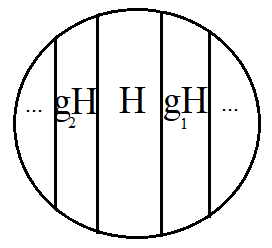
\includegraphics[width=0.4\linewidth]{Pic1}
		\end{figure}
		
		$|KH| = \sin x,\ |LA| = \tg x,\ S_{OAK} = 0.5 \cdot OA \cdot KH = 0.5 \cdot \sin x, S_{sectKOA} = 0.5 \cdot (OA)^2 \cdot x = 0.5 \cdot x, S_{OAL} = 0.5 \cdot OA \cdot LA = 0.5 \cdot \tg x$. \\
		\\
		$S_{OAK} < S_{sectKOA} < S_{OAL} \Rightarrow \sin x < x < \tg x$. \\
		\\
		Так как $\sin x > 0$, можем разделить на него. $1 < \frac{x}{\sin x} < \frac{1}{cosx} \Leftrightarrow 1 > \frac{\sin x}{x} > cosx$. По лемме о двух полицейских $\frac{\sin x}{x} \rightarrow 1, x \rightarrow 0$. \\
		
		\subsection{22}
		1) \textbf{Непрерывность экспоненты (в любой точке $a \in \mathbb{C}$)}\\
		\\
		Пусть $a = 0$. $\lim_{x \to 0} \exp(x) = 1 + \lim_{x \to 0} x \cdot \lim_{x \to 0} \frac{\exp(x) - 1}{x} = 1 + 0 \cdot 1 = 1 = \exp(0)$ -- непрерывность доказана. \\
		\\
		Для произвольного a получим $\lim_{x \to a} \exp(x) = \lim_{y \to 0} \exp(a + y) = \lim_{y \to 0} \exp(a) \cdot \exp(x) = \exp(x) \cdot \lim_{y \to 0} \exp(x) = \exp(a)$. \\
		\\
		2) \textbf{Существование и непрерывность логарифма}\\
		\\
		Существует функция $\ln : (0, +\infty) \rightarrow \mathbb{R}$, обратная к $\exp$ на действительной оси: $\ln (\exp) = x, \exp(\ln (y)) = y \forall x \in \mathbb{R}, y \in (0, +\infty)$. \\
		\\
		Доказательство. Так как функция $\exp(x)$ при $x \in \mathbb{R}$ строго возрастает и ее множество значений состоит из всех положительных чисел (*), $\forall y \in (0, +\infty) \ \exists ! x \in \mathbb{R}$, для которого $y = \exp(x)$ -- существование доказано, единственность следует из строгой монотонности. Положим $\ln y = x$ по определению. \\
		\\
		(*) Функция $\exp(x)$ при $x \in \mathbb{R}$ строго возрастает и ее множество значений состоит из всех положительных чисел. \\
		\\
		Доказательство. Так как $\exp(x + y) = \exp(x) \cdot \exp(y) \; \forall x, y \in \mathbb{C}$, $1 = \exp(0) = \exp(x - x) = \exp(x) \cdot \exp(-x)$, то есть $\exp(-x) = \frac{1}{\exp(x)}$. Значит, $\exp(x) \neq 0$ (в т.ч. $\forall x \in \mathbb{C}$).\\ 
		\\
		Рассматриваем $x \in \mathbb{R}$. $\exp(x) = \exp(\frac{x}{2} + \frac{x}{2}) = \exp(\frac{x}{2})^2 > 0$. \\
		\\
		$\exp(x) > x + 1 \ \forall x > 0$, так как $\exp(x) = e^x = 1 + x + \frac{x^2}{2} + ... > 1 + x$. \\
		\\
		$\Rightarrow$ по лемме о двух полицейских (? -- нет оценки сверху) $\lim_{x \to \infty} \exp(x) = +\infty$. Так как $\lim_{x \to -\infty} e^x = \lim_{y \to +\infty} e^(-y) = \lim_{y \to +\infty} \frac{1}{e^{y}} = 0$. То есть среди значений $\exp(x)$ на действительной оси есть сколь угодно близкие к нулю и сколь угодно большие числа. Из теоремы о промежуточном значении функция принимает все положительные значения $y$. \\
		\\
		Если $y > x$, $\exp(y) = \exp(x) \cdot \exp(y - x) > \exp(x)(1 + y - x) > \exp(x) \Rightarrow$ на действительной оси функция строго монотонна. \\
		
		\subsection{23}
		